\documentclass[10pt,a4paper,twocolumn]{article}
\usepackage[font=small,skip=0pt]{caption}

%\renewcommand{\section}{\section{\bold{#1}}

\newcommand{\blankpage}{
\newpage
\thispagestyle{empty}
\mbox{}
\newpage
}

\usepackage[colorlinks=false]{hyperref}
\hypersetup{%
  colorlinks = true,
  linkcolor  = black
}
\usepackage{geometry}
\usepackage{url}
\usepackage{booktabs}

% maths
\usepackage{bm}
\usepackage{xspace}

% algorithms
\usepackage{algorithm,algpseudocode}
\newcommand{\init}{\textbf{Init}\xspace}
\newcommand{\dokw}{\textbf{do}\xspace}
\newcommand{\upon}{\textbf{Upon}\xspace}
\newcommand{\interface}{\textbf{Interface}\xspace}
\newcommand{\crash}{\textbf{Crash}\xspace}
\newcommand{\eventname}{\textbf{EventName}\xspace}
\newcommand{\procname}{\textbf{ProcName}\xspace}
\newcommand{\timename}{\textbf{TimeName}\xspace}
\newcommand{\state}{\textbf{State}\xspace}
\newcommand{\trigger}{\textbf{Trigger}\xspace}
\newcommand{\requests}{\textbf{Requests}\xspace}
\newcommand{\indications}{\textbf{Indications}\xspace}
\newcommand{\proc}{\textbf{Procedure}\xspace}
\newcommand{\timer}{\textbf{Timer}\xspace}
\newcommand{\call}{\textbf{Call}\xspace}
\newcommand{\return}{\textbf{Return}\xspace}
\newcommand{\setup}{\textbf{Setup}\xspace}
\newcommand{\periodic}{\textbf{Periodic}\xspace}
\newcommand{\cancel}{\textbf{Cancel}\xspace}
\newcommand{\receive}[3]{\textbf{Receiver} (\textbf{#1}, \emph{sender}, #2, #3)}
\newcommand{\send}[3]{\textbf{Send} (\textbf{#1}, \emph{dest}, #2, #3)}
\algblockdefx{Interface}{EndInterface}[1]{\interface #1}{\textbf{end} \interface}
\algblockdefx{AlgState}{EndAlgState}[1]{\state #1}{\textbf{end} \state}
\algblockdefx{Requests}{EndRequests}{\requests\textbf{:}}{}
\algblockdefx{Indications}{EndIndications}{\indications\textbf{:}}{}
\algblockdefx{Upon}{EndUpon}[1]{\upon #1 \algorithmicdo}{\textbf{end} \upon}
\algblockdefx{Trigger}{EndTrigger}[1]{\trigger #1}{\textbf{end} \trigger}
\algrenewcommand\textproc{}
\algrenewcommand\algorithmicprocedure{\textbf{Procedure}}
\makeatletter
\newlength{\trianglerightwidth}
\settowidth{\trianglerightwidth}{$\triangleright$~}
\algnewcommand{\LineComment}[1]{\State \texttt{//} \textit{#1}}
\algnewcommand{\LineCommentCont}[1]{\State%
  \parbox[t]{\dimexpr\linewidth-\ALG@thistlm}{\hangindent=\trianglerightwidth \hangafter=1 \strut$\triangleright$ \emph{#1}\strut}}
\makeatother
\newcommand{\farg}[1]{\ensuremath{\textbf{arg}_{#1}}\xspace}

% % Fonts
\usepackage{times}
\usepackage[T1]{fontenc}

\def\course{Cloud Computing Systems}
\def\coursePT{Sistemas de Computação Cloud}

\def\titulo{TuKano Implementation leveraging Kubernetes}
\title{\titulo}

\def\data{\today}
\date{\data}



% Set your name here
\def\name{Filipe Colla David and Victor Ditadi}
\def\institution{
Departamento de Inform{\'a}tica\\
Faculdade de Ciências e Tecnologia\\
Universidade NOVA de Lisboa}

\author{\name\\ \institution}

% The following metadata will show up in the PDF properties
\hypersetup{
  colorlinks = true,
  urlcolor = black,
  pdfauthor = {\name},
  pdfkeywords = {Pseudocode, Link Abstractions}
  pdftitle = {\course: Lab 1 Problem},
  pdfsubject = {\course},
  pdfpagemode = UseNone
}

\geometry{
  body={6.5in, 9.0in},
  left=1.0in,
  top=1.0in
}

% Customize page headers
\pagestyle{myheadings}
\markright{\course - Project TuKano Kubernetes Report}
\thispagestyle{empty}

% Custom section fonts
\usepackage{sectsty}

\usepackage{amsmath}
\usepackage{listings}
\usepackage{graphicx}

\sectionfont{\rmfamily\mdseries\Large\textbf}
\subsectionfont{\rmfamily\mdseries\itshape\large}

\begin{document}

\pagenumbering{arabic} 

\maketitle

\section{Introduction}
\label{sec:intro}
This document explains the implementation of the TuKano App leveraging Kubernetes{\cite {kubernetes}}. TuKano is a social network inspired in existing video sharing services, such as TikTok or Youtube Shorts. TuKano users can upload short videos to be viewed (and liked) by other users of the platform. The social network aspect of TuKano resides on having users follow other users, as the main way for the platform to populate the feed of shorts each user can visualize.
\par The implementation of the application is divided will be divided into several microservices that will be managed by a Kubernetes Cluster. The performance analysis of using the different services will be presented in Section \ref{sec:Perf}.

\section{TuKano Application}
\label{sec:application}
This application can be divided basically into three major logical components, Users, Shorts and Blobs. 
\par The Users component holds all the logic for creating a user, deleting a user.
\par The Shorts component holds all the logic for creating, deleting a Short. A Short is a data model that holds the information for regarding a specific video, that was uploaded to the application. This component also contains the logic for following and liking other users/shorts.
\par The Blobs component holds all the logic for creating, deleting a blob.
\par These components are all related, however there's a stronger correlation between a Short and Blob, since every short contains the URL for a specific blob.

\section{Architecture and Behavior}
\label{sec:architecture}
This application is contained inside a Kubernetes Cluster, which manages the deployment, scaling, and operation of the microservices. As mentioned in the introduction, the application was divided into several microservices. 
\subsection{Components, Microservices}
As shown in Figure \ref{fig:tukano_architecture}, there are 5 major logical components, they are all defined as microservices, except for the ConfigMap, which complements the functionality of these microservices, additionally each one has a service to allow them to be reached via a DNS entry, managed by the Kubernetes Control Plane, instead of using the private cluster IpAddress of that instance.
\subsubsection{MINIO Service}
Minio\cite{minio} is a high-performance, distributed object storage system. It is designed to handle large amounts of unstructured data, such as photos, videos, log files, backups, and container images, which makes it a perfect replacement for Azure Blob Storage. It has a PVC (persistent volume claim) attached to avoid losing any data in the event of a restart of this deployment and contains a LoadBalancer that exposes this microservice to the outside of the cluster.

\subsubsection{PostgreSQL}
This microservice serves as the main database of the application, where user, shorts, following, and likes information is stored. It is defined as a StatefulSet, which is common practice in the industry. It also has a PVC attached to prevent data loss in the event of a StatefulSet restart.

\subsubsection{Redis Cache}
This microservice is used to cache frequently accessed information and cookies for user authentication.

\subsubsection{ConfigMap}
This is an individual resource that holds all the necessary environmental variables for the application.

\subsubsection{TuKano RestAPI}
This is a microservice containing the central REST API of this application. It holds the logic for creating and removing users, managing shorts, and storing blobs.
\par This microservice, in its essential form, consists of a pod with a Docker container that runs the Docker image defined in the repository of this project. This Docker image is built on top of \verb|tomcat:10.0-jdk17-openjdk-slim|, which allows it to run a Tomcat webserver that exposes a specific port for communication.
\par The communication with the database is handled using an Hibernate configuration and a JDBC Driver\cite{jdbc}. Communication with the MINIO storage is achieved through a MINIO Client\cite{minioClient}. Finally, uses Jedis\cite{jedis}, a Java client for Redis Cache, to interact with the caching service.


\subsection{Automated Deployment}
\label{sec:automatedDepl}
In order to easily deploy this application, a Makefile program was developed. A deployment of an application like this, requires several steps, and doing it manually is error prone.
The process:
\begin{enumerate}
  \itemsep0em 
  \item Compile the TuKano Application;
  \item Build the docker image and push it to the DockerHub;
  \item Update the docker image on the TuKano microservice yaml definition;
  \item Deploy every microservice available.
\end{enumerate}
As mentioned previously this process is mostly automated, however, there are some values from the ConfigMap that must be changed manually.

\subsection{Behavior}
\label{sec:behaviour}
Each microservice, upon starting will have access to the "Secrets" ConfigMap that holds all the necessary environmental variables for the configuration of their state. This includes the connections strings to the Database, Cache and Minio Storage, as well as some passwords and additional configuration parameters. However, as previously mentioned, there is a parameter on the ConfigMap that must be changed, the external URL of the MINIO LoadBalancer. Since the attribution of this URL is dynamic, this manual extra step is needed in order to ensure that the shorts will be stored with the right address to its blob. This is achieved by editing the "Secrets" ConfigMap, and deleting the TuKano RestAPI pod afterwards, so that it updates it's values from the new ConfigMap.
\par Once this initial configuration is complete, the application is ready to accept requests. As shown in Figure \ref{fig:tukano_architecture}, the TuKano Rest API is the central communication of the whole ecosystem, it communicates with the Database and the Cache to store the relational information of the users activity, and communicates with the MINIO storage microservice to store the blobs. The MINIO makes this blobs available through a LoadBalancer that exposes the service to the outside of the Kubernetes cluster.

\section{Performance Analysis}
\label{sec:Perf}
In this section there will be an analysis of the performance. The performance analysis will be done with the framework Artillery\cite{artillery}, that allows the programmer to test its application by creating several HTTP requests, once the experiment with the configured HTTP requests terminates, the framework outputs several statistics with the results obtained from the experiment.
\par The performance analysis will simulate a realistic flow of data over different configurations of the application:
\begin{itemize}
  \item \textbf{Locally:} With Cache vs No cache, single instance of each microservice locally.
\end{itemize}
This scenario consists in making several HTTP requests to the application to test all endpoints, this are over the span of 10 seconds, starting with one client/second ramping up to five clients/second.


\subsection{Locally}
\label{sec:realisticFlow}
From the Figure \ref{fig:performance_analysis} we can observe that both configurations, had the roughly the same amount of status codes, which is a good indication that both are well configured, additionally, \ref{fig:ResponseTimes} we can see that using cache improves the response times, as excepted.
\begin{figure}[h]
  \centering
  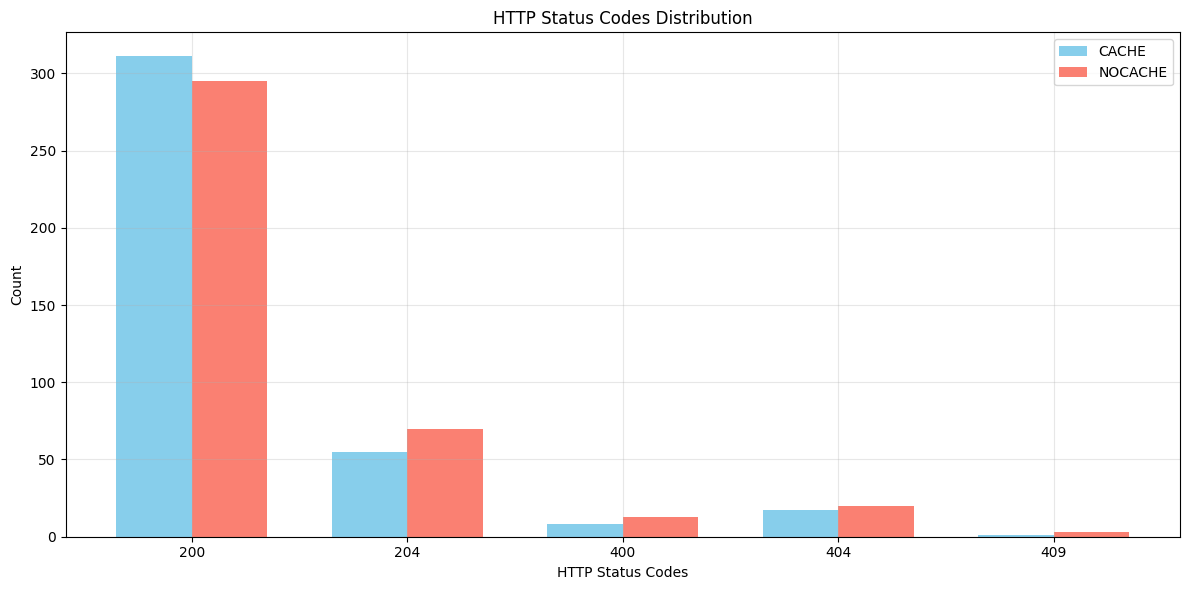
\includegraphics[width=0.5\textwidth]{images/HTTPStatusCodeDistribution.png}
  \caption{Performance Analysis Results}
  \label{fig:performance_analysis}
\end{figure}
\begin{figure}[h]
  \centering
  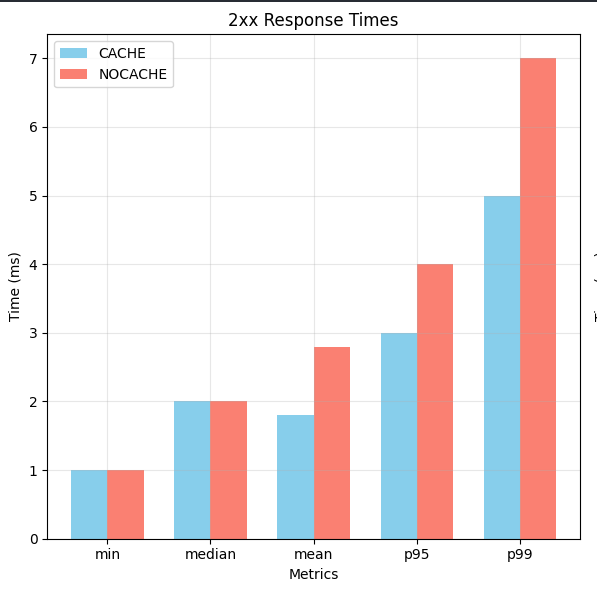
\includegraphics[width=0.5\textwidth]{images/ResponseTimes.png}
  \caption{Response Times of }
  \label{fig:ResponseTimes}
\end{figure}

\section{Future Work}
\label{sec:FutWork}
As for future work, the main thing needed would be to change the ConfigMap that holds all the information for the microservices, including the passwords to a Kubernetes Secret, which much more secure for sharing sensitive information.

\section{Challenges and Limitations}
\label{sec: challengesLimit}
The project well when in deployed locally in Minikube, however some issues with persistent volumes and available nodes occurred when deploying to Azure IaaS.

\section {Conclusions}
\label{sec:Conc}
\par When deploying microservices to Kubernetes, there is an initial definition of each individual microservice, when compared to SaaS, the code just needs to ready to connect to the already existing services.
\par However, development with Kubernetes is much faster using Azure SaaS, by using Minikube locally.

\appendix
\section{Appendix}
\begin{figure*}[h]
  \centering
  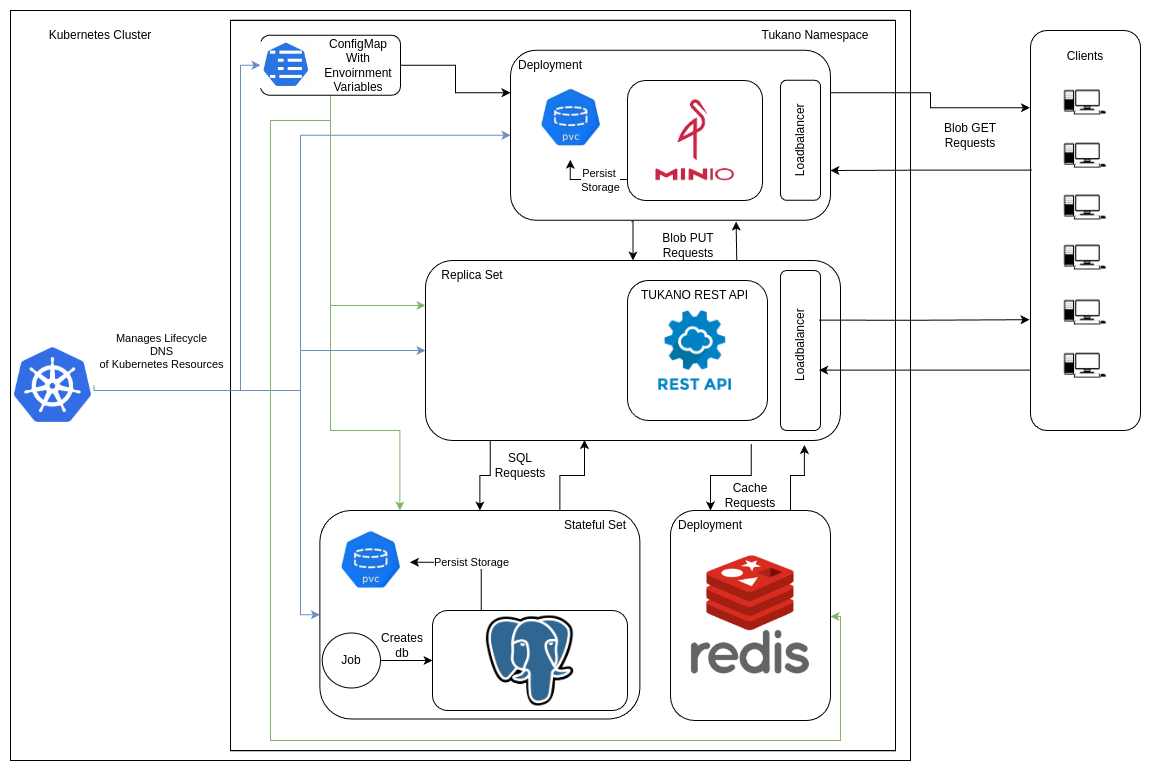
\includegraphics[width=\textwidth]{images/TuKanoArch.png}
  \caption{TuKano Application Architecture}
  \label{fig:tukano_architecture}
\end{figure*}

\bibliography{biblio}
\bibliographystyle{abbrv}

\end{document}